\documentclass{article}
% ========================
% = document information =
% ========================
\title{An Overview of Two Approaches for Knowledge Representation and Reasoning in the Context of Planning}
\author{Gregory Gelfond and Glen Hunt}
\date{\today}

% =================================
% various useful packages
% =================================

\usepackage{listings}
\usepackage{amsmath}
\usepackage{amssymb}
\usepackage{amsthm}
\usepackage{ccfonts}
\usepackage{euler}
\usepackage{graphicx}
\usepackage[T1]{fontenc}
\usepackage[scaled]{beramono}
\usepackage[utf8]{inputenc}
\usepackage[english]{babel}
\usepackage[parfill]{parskip}
\usepackage[usenames,dvipsnames]{color}
\usepackage[top=1in,bottom=1in,left=1in,right=1in,includehead,includefoot,letterpaper]{geometry}
\usepackage{tabularx}
\usepackage{booktabs}

% ==========
% = colors =
% ==========
\definecolor{LightGray}{gray}{.5}
\definecolor{LighterGray}{gray}{.75}
\definecolor{IdentifierGray}{gray}{.2}

% ======================
% = listing appearance =
% ======================
\lstset{
basicstyle=\footnotesize\ttfamily,
keywordstyle=\color{MidnightBlue},
commentstyle=\color{LightGray}\itshape,
stringstyle=\color{OliveGreen},
emph={True,False,None},
emphstyle=\color{RedOrange},
identifierstyle=\color{IdentifierGray},
numbers=left,
numberstyle=\tiny\ttfamily\color{LighterGray},
numbersep=10px,
breaklines=true,
breakatwhitespace=true,
showstringspaces=false,
frame=single
}

% =================================
% mathematical notation
% =================================

\newtheorem{theorem}{Theorem}
\newtheorem{lemma}[theorem]{Lemma}
\newtheorem{proposition}{Proposition}
\newtheorem{example}{Example}
\newtheorem{definition}{Definition}
\newtheorem{observation}{Observation}
\newtheorem{corollary}{Corollary}


\newcommand{\pair}[2]{\ensuremath{(#1, #2)}}
\newcommand{\triple}[3]{\ensuremath{(#1, #2, #3)}}
\newcommand{\union}{\ensuremath{\cup}}
\newcommand{\intersection}{\ensuremath{\cap}}
\newcommand{\conj}{\ensuremath{\wedge}}
\newcommand{\disj}{\ensuremath{\vee}}
\newcommand{\impl}{\ensuremath{\Rightarrow}}
\newcommand{\eqvl}{\ensuremath{\Leftrightarrow}}
\newcommand{\entails}{\ensuremath{\models}}
\newcommand{\ktimes}{\ensuremath{\otimes}}
\newcommand{\AL}{\ensuremath{\mathcal{AL}}}

% =================================
% action language notation
% =================================

\newcommand{\dynamiclaw}[2]{\ensuremath{#1 \: \mathbf{causes} \: #2}}
\newcommand{\dynamiclawp}[3]{\ensuremath{#1 \: \mathbf{causes} \: #2 \: \mathbf{if} \: #3}}
\newcommand{\staticlaw}[2]{\ensuremath{#1 \: \mathbf{if} \: #2}}
\newcommand{\initially}[1]{\ensuremath{\mathbf{initially} \: #1}}
\newcommand{\impossible}[2]{\ensuremath{\mathbf{impossible} \: #1 \: \mathbf{if} \: #2}}
\newcommand{\sense}[2]{\ensuremath{#1 \: \mathbf{determines} \: #2}}
\newcommand{\maysense}[2]{\ensuremath{#1 \: \mathbf{may \: determine} \: #2}}
\newcommand{\announce}[2]{\ensuremath{#1 \: \mathbf{announces} \: #2}}
\newcommand{\observes}[3]{\ensuremath{#1 \: \mathbf{observes} \: #2 \: \mathbf{if} \: #3}}
\newcommand{\observesu}[2]{\ensuremath{#1 \: \mathbf{observes} \: #2}}
\newcommand{\observesp}[3]{\ensuremath{#1 \: \mathbf{partially \: observes} \: #2 \: \mathbf{if} \: #3}}

% =====================================
% = bold font fix when using concrete =
% =====================================
\renewcommand{\bfdefault}{sbc}

\begin{document}
\maketitle

\section{Introduction}

Dijkstra viewed programming as the process of the ``refinement of specification.'' This applies not only to imperative programming, but in the myriad fields of Artificial Intelligence Research. It is especially made clear given that the levels of refinement we are able to obtain in our various formalisms, programs, etc.\, are inherently tied to the languages we use to reason about our problem domains.

This is also a central view taken by many members of what has been termed: the ``Knowledge Representation and Reasoning Community.'' Within this community one of the central goals has been to understand and formalize the reasoning of intelligent agents. A number of languages have developed such \emph{action languages}, and the language of \emph{answer set prolog} (denoted throughout as A-Prolog). A rather significant body of work has been done regarding various reasoning tasks such as planning, diagnosis, prediction, counter-factual reasoning, etc., all from the perspective of them being simply one of many reasoning tasks an agent may perform. This has lead to a framework for the design and development of intelligent agents based on a \emph{portfolio} of languages, corresponding roughly to individual levels of refinement about an agent's knowledge of the domain.

This central view does not appear to be shared by the ``Classical Planning'' community, given its use of a single language, \emph{PDDL}, which was ``originally developed by the AIPS-98 Competition Committee for use in defining problem domains.''

This difference in first principles leads to some interesting consequences which we hope to explore to some extent in this paper. The rest of this paper is structured as follows: an overview of the classical planning approach will be given in the context of four different planning domains, The Blocks World, Towers of Hanoi, Lin's Briefcase, and an Electrical Circuit. Once this has been, a similar overview of the knowledge representation and reasoning approaches, including descriptions of the action language $\AL$, followed by the logic programming language of A-Prolog. Once this has been covered, representations of the aforementioned domains will be presented.

\section{Classical Planning Overview}
\subsection{Background}
Planning, in general, consists of computing a sequence of actions which, starting in an initial state or states, will achieve a set of goal states. Classical planning, then, is a constrained planning task, which is fully observable, deterministic, finite, static (i.e. the world does not change unless the agent acts), and discrete (i.e. time, actions, objects and effects are not continuous). Nonclassical planning, by contrast, is used to describe planning in partially observable or stochastic environments. 

% TODO: add appropriate subsection break here
\subsubsection{Difficulties of Classical Planning}

Typical problem-solving agents which make use of standard search algorithms (i.e. depth-first, breadth-first, $A^*$, etc) encounter several difficulties when solving classical planning problems; each of these must be kept in mind when designing a planning agent. First of all, the agent may be overwhelmed by ``irrelevant'' actions (that is, actions which do not necessarily bring the agent closer to achieving a goal). There are multiple ways within the classical planning community of discouraging a planning agent from considering irrelevant actions; the use of regression search, for example, is one way to attempt to handle this problem. 

Another difficulty in classical planning is finding a good heuristic function. Because a problem-solving agent would see the goal state only as a ``black box'' which is either true or false for a given state, it would require a new heuristic for each specific problem it encounters. A planning agent, however, may have access to a representation of the goal state as a conjunction of subgoals, in which case it can use a single domain-independent heuristic; namely, the number of unsatisfied conjuncts. 

Similarly, a problem-solving agent might be inefficient because of its inability to take advantage of problem decomposition. A planning agent which views a state as a conjunction of literals, however, might be able to decompose the goal into a conjunction of subgoals, and then attempt to find a plan to achieve each subgoal. There are tradeoffs to this approach, however. Even if a planning agent can work on subgoals independently, some additional work may be required to combine the resultant subplans. Additionally, for some domains, on one subgoal may undo another.

% TODO: add appropriate subsection break here
\subsubsection{Representing Classical Planning Problems}

Classical planning problems are represented using three formalisms: states, goals and actions. These constructs form the basis of the languages used to encode planning problems in such a way that planners can understand them and operate on them to search for plans. 

States in classical planning problems 

\subsection{PDDL}
The Planning Domain Definition Language, or PDDL, is the lingua franca in the classical planning community. It was originally developed by the Artificial Intelligence Planning Systems 1998 Competition Committee for use in defining problem domains. It is not as expressive as some other languages which may be used for planning; however, this is by design, as the planning community wanted the language to be as simple and efficient as possible. Because it was designed for use in an international planning competition, development of the syntax and semantics of PDDL has been largely tied to various competitions. As a result, the development of planners which are able to execute PDDL code to search for plans has been somewhat piecemeal with respect to the formal language specification. That is, particular planners submitted to these competitions may only implement a subset of the features given in the language specification of PDDL. 

A particularly striking example of the conflict between the need for PDDL to be simple (so that it may be efficiently parsed) and the desire for it to be expressive may be found in the case of PDDL axioms. Axioms allow for the derivation of some derived predicates, whose value in there current state depends upon some basic predicates (under the closed-world assumption). In \cite{Thiebaux:2003ys}, it is argued that these axioms not only aid the expressiveness of the language, but also suggests that adding a reasonable implementation which could handle these axioms is beneficial for performance. In many of the domains we discuss in Section~\ref{sub:planning_domain_examples}, the ability to use these axioms could have significantly simplified our representation of the problem and domain.
 

\subsection{FF Planner}
In order to test the PDDL code we wrote for each of our test domains, we needed to decide on a planner to use. We selected Fast-Forward (FF), because it was simple to compile and run on our systems, and it supported most of the features of PDDL we wanted to be able to take advantage of when encoding the test domains. Most of the information in this section comes from \cite{Hoffmann:2001fk}.

FF was the most successful automatic planner in the AIPS-2000 planning systems competition. However, the general idea behind FF was not new to the classical planning community - the basic principle is actually the same as that of the Heuristic Search Planner (HSP). FF executes a forward search in the state space, guided by a heuristic which is extracted from the domain description automatically. This function is extracted by relaxing the planning problem; a part of the specification (specifically, the delete lists of all actions) is ignored. 

There are a number of details in which FF is different from its predecessor, HSP:
\begin{enumerate}
    \item FF makes use of a more sophisticated method of heuristic evaluation, which takes into account positive interactions between facts.
    \item FF uses a different local search strategy; specifically, it is able to escape plateaus and local minima through the use of systematic search.
    \item FF includes a mechanism which identifies those successors of a search node which appear to be (and usually are) most helpful in achieving the goal. 
\end{enumerate}

The main difficulty which results from viewing domain independent planning as heuristic search is the automated derivation of the heuristic function. A common approach to this problem (which is adopted here) is to relax the general problem $\mathcal{P}$ into a simpler problem $\mathcal{P}^\prime$ which can be efficiently solved. Given a search state in the original problem, $\mathcal{P}$, the solution length of the same state $\mathcal{P}^\prime$ may be used to estimate the difficulty of $\mathcal{P}$. In \cite{Bonet:1997uq}, Bonet et al. propose a way to apply this idea to domain independent planning. In this paper, the high-level problem description is relaxed by ``ignoring'' delete lists. This means that in the relaxed problem, actions can only add new atoms to state - all negative literals in the effects of actions are ignored, and leave those literals in the state unchanged. As a result, states only grow (in terms of the number of literals present in the state) during execution of a sequence of such relaxed actions, and the problem is solved as soon as each goal literal has been added by some action. This relaxation can be used to derive heuristics that are informative on many benchmark domains in classical planning.

One such heuristic is the length of an optimal relaxed solution. This heuristic is admissible, and could be used to find optimal solution plans through application of $A^*$ search; however, computation of the length of an optimal relaxed solution is NP-hard \cite{Bylander:1994kx}. With this in mind, \cite{Bonet:1997uq} proposed a way of approximating relaxed solution length from a given search state $\mathcal{S}$, by computing weights over all facts which estimate their distance to $\mathcal{S}$. The key observation which lead to FF's heuristic method comes from \cite{Bylander:1994kx}: although computing optimal relaxed solution length is NP-hard, deciding relaxed solvability is actually in P. This means that there must exist polynomial-time decision algorithms, and if such an algorithm constructs a witness, that witness may be used for heuristic evaluation. One algorithmic method which accomplishes this is Graphplan, discussed in \cite{Blum:1997vn}. When applied to a solvable relaxed problem, Graphplan finds a solution in polynomial time. Facing a search state $\mathcal{S}$, therefore, FF runs a relaxed version of Graphplan starting at $\mathcal{S}$, and uses the resulting output for heuristic evaluation.

Although these heuristics can be computed in polynomial time, it is still costly to perform heuristic evaluation of states. A logical approach to this issue is to use hill-climbing as the search method, in order to attempt to reach the goal by evaluating as few states as possible. FF makes use of an enforced version of hill-climbing search. When facing a search state $\mathcal{S}$, FF evaluates all direct successors. If none of these successors has a better heuristic value than $\mathcal{S}$, the search then considers the next level (the successors' successors). Again, if none of the two-step successors looks better than $\mathcal{S}$, FF continues to the next level, and so on. This process ends when a state $\mathcal{S}^\prime$ which has a better heuristic evaluation than $\mathcal{S}$ is found. The path to $\mathcal{S}^\prime$ is then added to the current plan, and the search continues, starting at $\mathcal{S}^\prime$. If a planning problem does not contain dead end situations, this strategy is guaranteed to find a solution. 

\subsection{Planning Domain Examples}\label{sub:planning_domain_examples}
\subsubsection{Blocks World}

\subsubsection{Towers of Hanoi}

\subsubsection{Lin's Briefcase}

\subsubsection{Electrical Circuit}

\section{The Knowledge Representation and Reasoning Approach}

As was stated earlier, in the knowledge representation and reasoning community, the general approach is centered around the use of a portfolio of various knowledge representation languages, among which are the action language $\AL$, and the logic programming language A-Prolog. In keeping with the notion of programming as the refinement of specification we:
\begin{enumerate}
    \item Construct a mental model of the transition system described by the domain
    \item Describe the transition system via an \emph{action description} in some action language (such as $\AL$)
    \item Refine the action description further by translation into A-Prolog
\end{enumerate}
In this section we take a brief look at the languages $\AL$ and A-Prolog, and show their application towards the aforementioned domains.

\subsection{The Action Language $\AL$}

Simply put, action languages are a family of declarative languages designed for the purpose of describing the effects of actions. They have a simple syntax and semantics, while remaining powerful enough to represent many complex reasoning domains \cite{Bald2005}. Collections of statements are called \emph{action descriptions}, and define transitions whose nodes correspond to \emph{possible states of the world}\footnote{A difference we believe to be significant from the conception of a state in the classical view as simply an interpretation of the fluents present in a domain.}, and whose arcs are labeled by actions. An arc $\triple{\sigma}{\alpha}{\tau}$ states that if action $\alpha$ occurs in state $\sigma$, the resulting state will be $\tau$. In addition to specifying what changes due to the occurrence of a particular action, it is also vital to be able to specify what does not change. This is know as the \emph{frame problem} \cite{Shan97}, and its solution lies in an elegant and precise representation of what is called the \emph{inertia axiom}. The beauty and utility of such languages stems from the ability to compactly represent huge transition systems, and in their graceful approach towards solving the frame problem.

Action descriptions in the language of $\AL$ are collections of three statement types: \emph{dynamic causal laws}, \emph{static causal laws}, and \emph{impossibility conditions}. Dynamic causal laws are statements of the form:
\begin{align*}
    &\dynamiclawp{a}{f}{l_{0},\ldots,l_{n}}
\end{align*}
where $a$ is an action, and $f$, and $l_{0},\ldots,l_{n}$ are fluent literals. Laws of this form a read as: ``action $a$ causes $f$ to be come true if $l_{0},\ldots,l_{n}$.'' The corresponding arc in the transition diagram is shown in Figure~\ref{fig-dcl}.
\begin{figure}[htb]
    \centering
    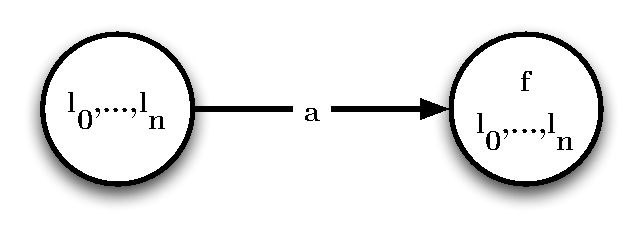
\includegraphics[scale=0.5]{dynamic-law}
    \caption{transition defined by a simple causal law}
    \label{fig-dcl}
\end{figure}

Static causal laws have the form:
\begin{align*}
    &\staticlaw{f}{l_{0},\ldots,l_{n}}
\end{align*}
where $f$, and $l_{0},\ldots,l_{n}$ are fluent literals. Such laws are read as: ``$f$ is true whenever $l_{0},\ldots,l_{n}$ are true.'' Unlike dynamic causal laws, static laws are used to describe the properties of states, as well as the \emph{indirect effects} of actions.
\begin{example}
{\rm
Consider the following action description $AD_{1}$:
\begin{align*}
    &\dynamiclaw{a}{f} \\
    &\staticlaw{g}{f}
\end{align*}
and let the state, $\sigma = \{\neg{f}, \neg{g}\}$. If $a$ is executed in $\sigma$, we have the transition depicted in Figure~\ref{fig-scl}.
\begin{figure}[htb]
    \centering
    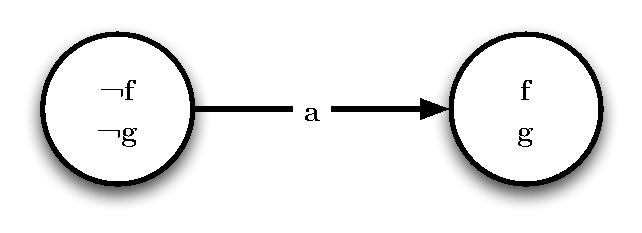
\includegraphics[scale=0.5]{static-law}
    \caption{transition involving both direct and indirect effects}
    \label{fig-scl}
\end{figure}
}
\end{example}

Impossibility conditions have the form:
\begin{align*}
    &\impossible{a}{l_{0},\ldots,l_{n}}
\end{align*}
where as before, $a$ is an action, and $l_{0},\ldots,l_{n}$ are fluent literals. Rules such as this are used to state that: ``action $a$ may not occur in a state which satisfies $l_{0},\ldots,l_{n}$.'' From the view of a transition system, this means that there are no outgoing arcs labeled by $a$ originating from a state which satisfies $l_{0},\ldots,l_{n}$.

The semantics of an action description of $\AL$ is given by its transition diagram. For a more detailed treatment, we refer the reader to \cite{Bald2005}. Having described the action language $\AL$, we now turn our attention to the language of A-Prolog.

\subsection{The Language of A-Prolog}

The language of A-Prolog is a logic programming language developed by Michael Gelfond and Vladimir Lifschitz in \cite{GL88}. It has a simple syntax, and is focused on modeling the beliefs of a rational agent. A rather broad community has developed around it, and it has emerged as strong programming paradigm in its own right.

A logic program in the language of A-Prolog is defined as a collection of rules of the form \cite{GL88,Baral03}:
\begin{align*}
    &l_{0} \leftarrow l_{1},\ldots,l_{m}, not \: l_{m+1}, \ldots, not \: l_{n}.
\end{align*}
where $0 \leq m \leq n$, each $l_{i}$ is a literal, and $not$ represents \emph{negation-as-failure} (also termed \emph{default negation}). Rules of this form are read as: ``if an agent believes $l_{1},\ldots,l_{m}$ to be true and has no reason to believe in $l_{m+1},\ldots,l_{n}$, then he believes $l_{0}$ to be true.''

The left-hand side of a rule is known as the \emph{head}, and the right-hand side is called the \emph{body}. Rules with empty heads are known as \emph{constraints}, while those with empty bodies are termed \emph{facts}.

The variables of a program $\Pi$ range over the set of ground terms of its signature $\sigma$. Programs which do not contain any variables are said to be \emph{ground}. A rule $r$ which does contain variables may be viewed as a shorthand form for the entire set of its ground instantiations. A \emph{definite rule} is a rule which does not contain any occurrences of default negation, and programs comprised solely of definite rules are called \emph{definite programs}.

Let $S$ be a set of ground literals. The body of a rule is satisfied by $S$ if $\{l_{m+1},\ldots,l_{n}\} \intersection S = \emptyset$ and $\{l_{1},\ldots,l_{m}\} \subseteq S$. A rule with a non-empty head is satisfied by $S$ if either its body is not satisfied by $S$ or $l_{0} \in S$. A constraint is satisfied by $S$ if its body is not satisfied by $S$.

Given an arbitrary program $\Pi$, and a set of ground literals, $S$, the \emph{reduct} of $\Pi$ with respect to $S$, denoted by $\Pi^{S}$ is the definite program obtained from $\Pi$ by:
\begin{enumerate}
    \item deleting all rules in $\Pi$ which $not \: l$ in the body, where $l \in S$
    \item removing all remaining occurrences of $not \: l$ from the bodies of the remaining rules
\end{enumerate}
A set of ground literals, $S$, is said to be an answer set of a logic program $\Pi$ if it satisfies the following:
\begin{enumerate}
    \item if $\Pi$ is a definite program then $S$ is a minimal set of literals satisfying all of the rules of $\Pi$
    \item if $\Pi$ is not a definite program the $S$ is an answer set of $\Pi$ if and only if $S$ is an answer set of $\Pi^{S}$
\end{enumerate}

The fact that a program can have multiple (or no) answer sets has given rise to an alternative method of solving problems through logic programming, called \emph{Answer Set Programming} (ASP) \cite{Marek99,Niemela99}. In this approach, we develop logic programs whose answer sets have a one-to-one correspondence with the solutions of the particular problem being modeled. Typically an ASP program consists of:
\begin{itemize}
    \item rules for the enumeration of possible solutions to a problem as \emph{candidate answer sets}
    \item constraints which remove candidates that do not correspond to solutions of the problem
\end{itemize}
In the context of planning, the ``planning module'' will serve to generate possible sequences of while the ``goal specification'' will prune those which fail to satisfy our goal. 

\subsection{Domains}

In this section we examine a number of planning and apply the knowledge representation and reasoning approach towards their resolution. All of the listings presented in this paper are in the input language of the clingo answer set programming system \cite{clingo}.

\subsubsection{Lin's Briefcase}

Consider a domain consisting of a briefcase with two latches. Flipping a closed latch causes it to be open, while flipping an open latch causes it to become closed. How do we represent this domain using the reasoning about actions approach?

We begin by constructing a mental model of the system, which involves the transition system shown in Figure~\ref{lin-tran}.

\begin{figure}[htb]
    \centering
    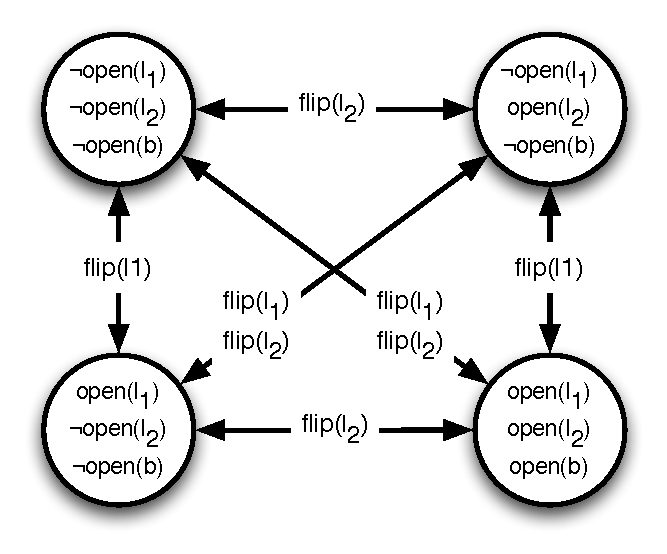
\includegraphics[scale=0.50]{briefcase}
    \caption{transition system for the Lin's Briefcase domain}
    \label{lin-tran}
\end{figure}

Once we have the transition fixed, we represent in in $\AL$ as follows:
\begin{align*}
    &\dynamiclawp{flip(l_{1})}{open(l_{1})}{\neg{open(l_{1})}} \\
    &\dynamiclawp{flip(l_{1})}{\neg{open(l_{1})}}{open(l_{1})} \\
    &\dynamiclawp{flip(l_{2})}{open(l_{2})}{\neg{open(l_{2})}} \\
    &\dynamiclawp{flip(l_{2})}{\neg{open(l_{2})}}{open(l_{2})} \\
    &\staticlaw{open(b)}{open(l_{1}),\:open(l_{2})} \\
    &\staticlaw{\neg{open(b)}}{\neg{open(l_{1})}} \\
    &\staticlaw{\neg{open(b)}}{\neg{open(l_{2})}}
\end{align*}

With our domain description in place, we translate the above laws and add some additional domain related information to obtain the following A-Prolog program:

\begin{lstlisting}[language=Prolog, caption=Lin's Briefcase Domain Description in A-Prolog, label=lst:asp-briefcase]
% ============================
% OBJECTS
% ============================

#const n = 2.

time(0..n).

latch(1).
latch(2).

% ============================
% FLUENTS
% ============================

fluent(open(Latch)) :-
	latch(Latch).

fluent(opened).

% ============================
% ACTIONS
% ============================

action(flip(Latch)) :-
	latch(Latch).

% ============================
% CAUSAL LAWS
% ============================

holds(open(Latch), T + 1) :-
	occurs(flip(Latch), T),
	-holds(open(Latch), T),
	latch(Latch),
	time(T).

-holds(open(Latch), T + 1) :-
	occurs(flip(Latch), T),
	holds(open(Latch), T),
	latch(Latch),
	time(T).

-holds(opened, T) :-
	-holds(open(Latch), T),
	latch(Latch),
	time(T).

holds(opened, T) :-
	not -holds(opened, T),
	time(T).

% ============================
% INERTIA AXIOMS
% ============================

holds(Fluent, T + 1) :-
    holds(Fluent, T),
    not -holds(Fluent, T + 1),
    fluent(Fluent),
    time(T).

-holds(Fluent, T + 1) :-
    -holds(Fluent, T),
    not holds(Fluent, T + 1),
    fluent(Fluent),
    time(T).

% ============================
% INITIAL STATE
% ============================

-holds(open(Latch), 0) :-
	latch(Latch).

% ============================
% GOAL SPECIFICATION
% ============================

goal(T) :-
	holds(opened, T),
	time(T).

done :-
	goal(T).

:- not done.

% ============================
% PLANNING MODULE
% ============================

1{occurs(Action,T) : action(Action)}1 :-
    not goal(T),
    time(T).

% ============================
% SOLVER DIRECTIVES
% ============================

#hide.
#show occurs(_,_).
\end{lstlisting}

\noindent Utilizing the clingo answer set solver we obtain the following two plans (this is due to the fact that the planning module is written in such a way as to only look for sequential plans, parallel plans may be supported through a minor modification):
\begin{verbatim}
Answer: 1
occurs(flip(2),1) occurs(flip(1),0) 
Answer: 2
occurs(flip(1),1) occurs(flip(2),0) 
SATISFIABLE

Models      : 2     
Time        : 0.000
  Prepare   : 0.000
  Prepro.   : 0.000
  Solving   : 0.000
\end{verbatim}

\subsubsection{Electrical Circuit}

We now turn our attention towards the representation of an electrical circuit domain. Such a domain is of interest due to the fact that there is essentially only a single action that an agent may perform, namely, the application of some input signals to the circuit. These signals must then be propagated throughout the entire circuit to obtain some output value.

Consider the electrical circuit shown in Figure~\ref{circuit}. Once a signal has been applied to inputs $1,2,3$, it must be propagated to the next level of the circuit within the same state. Static causal laws shine here.

\begin{figure}[htb]
    \centering
    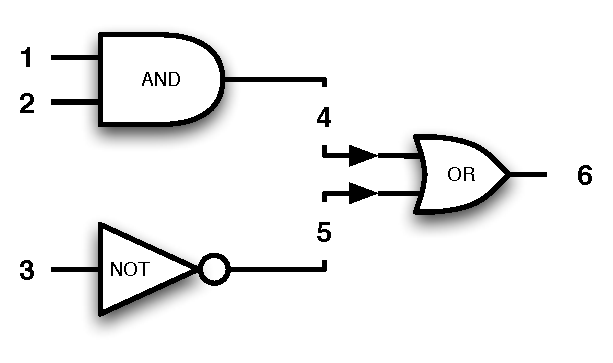
\includegraphics[scale=0.50]{circuit}
    \caption{a simple electrical circuit}
    \label{circuit}
\end{figure}

\begin{lstlisting}[language=Prolog, caption=Electrical Circuit Domain Representation in A-Prolog, label=lst:asp-circuit]
% ============================
% OBJECTS
% ============================

time(0).

% ============================
% CIRCUIT STRUCTURE
% ============================

wire(1..6).
gate(1..3).
and(1).
inverter(2).
or(3).

% and gate has inputs 1 and 2

input_to(1,1..2).

% inverter has input 3

input_to(2,3).

% or gate has inputs 4 and 5

input_to(3,4..5).

% and gate has output 4

output_from(1,4).

% inverter has output 5

output_from(2,5).

% or gate has output 6

output_from(3,6).

% ============================
% GENERAL DESCRIPTION OF GATES
% ============================

h(val(OUTPUT_WIRE, 1), T) :- 
    output_from(GATE, OUTPUT_WIRE),
    and(GATE),
    input_to(GATE, INPUT1),
    input_to(GATE, INPUT2),
    INPUT1 != INPUT2,
    h(val(INPUT1, 1), T),
    h(val(INPUT2, 1), T),
    time(T).

h(val(OUTPUT_WIRE, 0), T) :- 
    output_from(GATE, OUTPUT_WIRE),
    and(GATE),
    input_to(GATE, INPUT),
    h(val(INPUT, 0), T),
    time(T).
    
h(val(OUTPUT_WIRE, 0), T) :- 
    output_from(GATE, OUTPUT_WIRE),
    or(GATE),
    input_to(GATE, INPUT1),
    input_to(GATE, INPUT2),
    INPUT1 != INPUT2,
    h(val(INPUT1, 0), T),
    h(val(INPUT2, 0), T),
    time(T).

h(val(OUTPUT_WIRE, 1), T) :- 
    output_from(GATE, OUTPUT_WIRE),
    or(GATE),
    input_to(GATE, INPUT),
    h(val(INPUT, 1), T),
    time(T).
    
h(val(OUTPUT_WIRE, 1), T) :-
    output_from(GATE, OUTPUT_WIRE),
    inverter(GATE),
    input_to(GATE, INPUT),
    h(val(INPUT, 0), T),
    time(T).

h(val(OUTPUT_WIRE, 0), T) :-
    output_from(GATE, OUTPUT_WIRE),
    inverter(GATE),
    input_to(GATE, INPUT),
    h(val(INPUT, 1), T),
    time(T).

% ============================
% INITIAL STATE
% ============================
    
h(val(1, 1), 0).
h(val(2, 0), 0).
h(val(3, 1), 0).

% ============================
% SOLVER DIRECTIVES
% ============================

#hide.
#show h(_,_).
\end{lstlisting}

\subsubsection{Towers of Hanoi}

\begin{lstlisting}[language=Prolog, caption=Towers of Hanoi Domain Representation in A-Prolog, label=lst:asp-hanoi]
% ============================
% OBJECTS
% ============================

#const n = 7.

time(0..n).

disc(1).
disc(2).
disc(3).

peg(p1).
peg(p2).
peg(p3).

location(X) :- peg(X).
location(X) :- disc(X).

% ============================
% FLUENTS
% ============================

fluent(on(Disc,Location)) :-
    disc(Disc),
    location(Location),
    Disc != Location.

fluent(clear(Location)) :-
    location(Location).

% ============================
% ACTIONS
% ============================

action(move(Disc,Source,Destination)) :-
    disc(Disc),
    location(Source),
    location(Destination),
    Source != Destination.

% ============================
% CAUSAL LAWS
% ============================

holds(on(Disc,Destination), T + 1) :-
    occurs(move(Disc,Source,Destination), T),
    disc(Disc),
    location(Source),
    location(Destination),
    time(T).

-holds(on(Disc,Source), T + 1) :-
    occurs(move(Disc,Source,Destination), T),
    disc(Disc),
    location(Source),
    location(Destination),
    time(T).

:- occurs(move(Disc,Source,Destination), T),
   not holds(on(Disc,Source), T),
   disc(Disc),
   location(Source),
   location(Destination),
   time(T).

:- occurs(move(Disc,Source,Destination), T),
   not holds(clear(Disc), T),
   disc(Disc),
   location(Source),
   location(Destination),
   time(T).

:- occurs(move(Disc,Source,Destination), T),
   not holds(clear(Destination), T),
   disc(Disc),
   location(Source),
   location(Destination),
   time(T).

:- occurs(move(Disc,Source,Destination), T),
   disc(Destination),
   Destination < Disc,
   disc(Disc),
   location(Source),
   location(Destination),
   time(T).

-holds(clear(Location), T) :-
    holds(on(Disc,Location), T),
    location(Location),
    disc(Disc),
    time(T).

holds(clear(Location), T) :-
    not -holds(clear(Location), T),
    location(Location),
    time(T).

% ============================
% INERTIA AXIOMS
% ============================

holds(Fluent, T + 1) :-
    holds(Fluent, T),
    not -holds(Fluent, T + 1),
    fluent(Fluent),
    time(T).

-holds(Fluent, T + 1) :-
    -holds(Fluent, T),
    not holds(Fluent, T + 1),
    fluent(Fluent),
    time(T).

% ============================
% INITIAL STATE
% ============================

holds(on(1,2), 0).
holds(on(2,3), 0).
holds(on(3,p1), 0).

% ============================
% GOAL SPECIFICATION
% ============================

goal(T) :-
    holds(on(1,2), T),
    holds(on(2,3), T),
    holds(on(3,p3), T),
    time(T).

done :-
    goal(T).

:- not done.

% ============================
% PLANNING MODULE
% ============================

1{occurs(Action,T) : action(Action)}1 :-
    not goal(T),
    time(T).

% ============================
% SOLVER DIRECTIVES
% ============================

#hide.
#show occurs(_,_).
\end{lstlisting}

\section*{Roles in the Project}
\begin{tabularx}{\textwidth}{lX}
    \textbf{Name} & \textbf{Contributions} \\ \toprule
    Gregory Gelfond & \begin{itemize}
        \item Read cited papers
        \item Wrote A-Prolog problem and domain encodings
        \item Compiled project presentation
        \item Wrote report introduction
        \item Wrote knowledge representation and reasoning section of the report
        \item Contributed to comparison and analysis of methodologies
    \end{itemize} \\ \midrule
    Glen Hunt & \begin{itemize}
        \item Read cited papers
        \item Contributed classical planning information to the project presentation
        \item Wrote PDDL problem and domain encodings
        \item Wrote classical planning section of the report
        \item Contributed to comparison and analysis of methodologies 
    \end{itemize} \\ 
\end{tabularx}

\begin{thebibliography}{2}

\bibitem{GL88}
Michael Gelfond and Vladimir Lifschitz.
The Stable Model Semantics for Logic Programming.
In Robert A.\, Kowalski and Kenneth Bowen, editors, Proceedings of the Fifth International Conference on Logic Programming, pages 1070{1080}, Cambridge, Massachusetts, 1988.
The MIT Press.

\bibitem{Baral03}
Chitta Baral.
Knowledge Representation, Reasoning, and Declarative Problem Solving.
Cambridge University Press, January 2003.

\bibitem{Bald2005}
Marcello Balduccini.
Answer Set Based Design of Highly Autonomous, Rational Agents.
PhD thesis, Texas Tech University, December 2005.

\bibitem{Shan97}
Murray Shanahan.
Solving the frame problem: A mathematical investigation of the commonsense law of inertia.
MIT Press, 1997.

\bibitem{Marek99}
Victor Marek and Mirek Truszczynski.
Stable models and an alternative logic programming paradigm.
The Logic Programming Paradigm, pp. 375–398, Springer, 1999.

\bibitem{Niemela99}
Ilkka Niemela.
Logic programming with stable model semantics as a constraint programming paradigm.
AMAI, 25(3,4), 1999.

\bibitem{clingo}
Martin Gebser, Roland Kaminski, et.\,al.\,
A User's Guide to gringo, clasp, clingo, and iclingo.
2010.

\bibitem{Blum:1997vn}
A.~Blum and M.~Furst.
\newblock Fast planning through planning graph analysis.
\newblock {\em Artificial Intelligence}, 90(1-2):279--298, 1997.

\bibitem{Bonet:1997uq}
B.~Bonet, G.~Loernics, and H.~Geffner.
\newblock A robust and fast action selection mechanism for planning.
\newblock In {\em AAAI-97}, pages 714--719. MIT Press, 1997.

\bibitem{Bylander:1994kx}
T.~Bylander.
\newblock The computational complexity of propositional STRIPS planning.
\newblock {\em Artificial Intelligence}, 69(1-2):165--204, 1994.

\bibitem{Hoffmann:2001fk}
J.~Hoffmann.
\newblock FF: The fast-forward planning system.
\newblock {\em AI Magazine}, 22(3):57--62, 2001.

\bibitem{Thiebaux:2003ys}
S.~Thi{\'e}baux, J.~Hoffmann, and B.~Nebel.
\newblock In defense of PDDL axioms.
\newblock {\em Artificial Intelligence}, 18:961--968, 2003.


\end{thebibliography}

\end{document}